\documentclass[11pt,a4paper]{article}

\usepackage[margin=1in]{geometry}
\usepackage[T1]{fontenc}
\usepackage{lmodern}
\usepackage{microtype}
\usepackage{graphicx}
\usepackage{amsmath,amssymb}
\usepackage{booktabs}
\usepackage{array}
\usepackage{float}
\usepackage{xcolor}
\usepackage{listings}
\usepackage{algorithm}
\usepackage{algpseudocode}
\usepackage{enumitem}
\usepackage{fancyhdr}
\usepackage[hidelinks]{hyperref}

\definecolor{accent}{RGB}{190,70,20}
\definecolor{codebg}{gray}{0.96}

\lstset{
  language=Python,
  basicstyle=\ttfamily\footnotesize,
  backgroundcolor=\color{codebg},
  keywordstyle=\color{accent}\bfseries,
  commentstyle=\color{gray}\itshape,
  frame=single,
  rulecolor=\color{black!20},
  breaklines=true,
  columns=fullflexible,
  showstringspaces=false,
}

\pagestyle{fancy}
\fancyhf{}
\lhead{CSE3121 -- Algorithmic Implementation}
\rhead{Genetic Algorithm for TSP}
\cfoot{\thepage}
\renewcommand{\headrulewidth}{0.4pt}

\setlength{\parskip}{0.5em}
\setlength{\parindent}{0pt}

\begin{document}

% ---------------------------------------------------------------- title page
\begin{titlepage}
  \centering
  \vspace*{0.5cm}
  \includegraphics[width=0.8\textwidth]{college_logo.jpg}\\[1.6cm]

  {\large Department of Computer Science and Engineering}\\[1.2cm]

  {\Large\bfseries Artificial Intelligence and Soft Computing (CSE3121)}\\[0.4cm]
  {\large Algorithmic Implementation of AI Approaches with Viva}\\[1.6cm]

  \rule{\textwidth}{1.2pt}\\[0.5cm]
  {\huge\bfseries Genetic Algorithm for the\\[0.2cm] Travelling Salesman Problem}\\[0.4cm]
  {\large A study on 15 Indian cities, validated against the exact optimum}\\[0.3cm]
  \rule{\textwidth}{1.2pt}\\[2cm]

  \begin{tabular}{rl}
    \textbf{Submitted by:}  & Shashwat Shikhar Dwivedi \\[4pt]
    \textbf{Roll No.:}      & 2427030605 \\[10pt]
    \textbf{Submitted to:}  & Dr.\ Neha Chaudhary
  \end{tabular}

  \vfill
  {\large Academic Year 2026--27}
\end{titlepage}

% ---------------------------------------------------------------- abstract
\begin{abstract}
This report presents an implementation of a Genetic Algorithm (GA) for the Travelling Salesman Problem (TSP)
over 15 Indian cities. Tours are encoded as permutations and evolved using tournament selection, Order
Crossover, inversion mutation and elitism. Because the instance is small enough, the exact optimum
(7478.9~km) is computed with the Held--Karp dynamic programme, which gives a ground truth for judging the GA.
Over 10 independent runs the GA reaches a mean tour length of 7526.9~km (0.6\% above optimal) and finds the
true optimum in 5 of 10 runs, whereas random search with the same evaluation budget is 32.8\% above optimal and
the nearest-neighbour heuristic is 22.6\% above. Experiments on mutation rate and population size show how
each parameter affects solution quality.
\end{abstract}

\tableofcontents
\newpage

% ---------------------------------------------------------------- 1
\section{Introduction}

\subsection{Problem statement}
Given a set of $n$ cities and the distance $d(i,j)$ between every pair, find the shortest closed route that
visits each city exactly once and returns to the start. For a tour $\pi=(\pi_1,\dots,\pi_n)$ the objective is
\[
  L(\pi)=\sum_{i=1}^{n} d\bigl(\pi_i,\pi_{(i \bmod n)+1}\bigr).
\]
For $n=15$ there are $(15-1)!/2\approx4.4\times10^{10}$ distinct tours, so exhaustive enumeration is impractical,
and the problem is NP-hard in general.

\subsection{Why a Genetic Algorithm}
A GA is a population-based metaheuristic inspired by natural selection. Instead of improving one solution it
maintains a population of candidates and repeatedly applies selection, crossover and mutation. The population
explores several regions of the search space in parallel, and recombination lets good partial routes from
different tours be combined.

\subsection{Objectives}
\begin{itemize}[nosep]
  \item Implement a GA for TSP from scratch in Python.
  \item Validate it against the exact optimum computed by Held--Karp.
  \item Compare it with random search and nearest-neighbour baselines.
  \item Study the effect of mutation rate and population size.
\end{itemize}

% ---------------------------------------------------------------- 2
\section{Methodology}

\subsection{Problem data}
The 15 cities are Delhi, Mumbai, Kolkata, Chennai, Bengaluru, Hyderabad, Ahmedabad, Pune, Jaipur, Lucknow, Bhopal,
Patna, Chandigarh, Guwahati and Kochi. Each is given by its latitude and longitude, and the distance between two
cities is the great-circle (haversine) distance
\[
  d = 2R\arcsin\sqrt{\sin^2\!\tfrac{\Delta\varphi}{2}+\cos\varphi_1\cos\varphi_2\sin^2\!\tfrac{\Delta\lambda}{2}},
  \qquad R = 6371~\text{km}.
\]
All pairwise distances are precomputed into a $15\times15$ matrix.

\subsection{GA design}
Table~\ref{tab:design} summarises the design, and the following subsections explain each choice.

\begin{table}[H]
\centering
\caption{GA design and parameters.}
\label{tab:design}
\begin{tabular}{@{}ll@{}}
\toprule
Component & Choice \\
\midrule
Chromosome & Permutation of city indices \\
Fitness & $1/L(\pi)$ (selection compares $L$ directly) \\
Selection & Tournament, size $k=5$ \\
Crossover & Order Crossover (OX1), probability 0.9 \\
Mutation & Segment inversion, probability 0.2 \\
Elitism & Best 2 individuals copied unchanged \\
Population size & 150 \\
Generations & 300 \\
\bottomrule
\end{tabular}
\end{table}

\paragraph{Encoding.}
A chromosome is a permutation of the integers $0,\dots,14$, so every chromosome is a valid tour. A binary
encoding would produce many invalid tours with repeated or missing cities.

\paragraph{Fitness.}
Fitness is $1/L$, so shorter tours score higher. Tournament selection only needs an ordering, so the
implementation compares tour lengths directly, which is equivalent.

\paragraph{Selection.}
Tournament selection draws $k=5$ individuals at random and returns the shortest tour among them. The tournament
size controls selection pressure: larger $k$ favours the fittest more strongly but risks premature convergence.

\paragraph{Order Crossover (OX1).}
Ordinary one-point crossover would duplicate some cities and drop others. OX1 copies a random slice from parent~1
and fills the remaining positions with the missing cities in the order they occur in parent~2, which always
yields a valid permutation. Example with cut positions 2--4:
\begin{center}
\begin{tabular}{@{}ll@{}}
Parent 1 & $[1,2,\mathbf{3,4,5},6,7,8]$ \\
Parent 2 & $[3,7,5,1,6,8,2,4]$ \\
Slice kept from parent 1 & $[3,4,5]$ \\
Remaining genes in parent 2 order & $[7,1,6,8,2]$ \\
Child & $[7,1,\mathbf{3,4,5},6,8,2]$
\end{tabular}
\end{center}

\paragraph{Mutation.}
Inversion reverses a random sub-route. It changes only two edges of the tour, a small local move similar to a
2-opt step, and keeps the tour valid. For example, inverting positions 2--5 of $[1,2,3,4,5,6,7,8]$ gives
$[1,2,6,5,4,3,7,8]$.

\paragraph{Elitism.}
The two best tours of each generation are copied unchanged into the next, so the best tour found never gets worse.

\subsection{Algorithm}
\begin{algorithm}[H]
\caption{Genetic Algorithm for TSP}
\begin{algorithmic}[1]
\State Initialise population $P$ of $N_p$ random permutations
\For{$g = 1$ \textbf{to} $G$}
  \State Evaluate tour length $L(\pi)$ for every $\pi\in P$
  \State Record the best tour found so far
  \State $P' \gets$ the $e$ best tours of $P$ \Comment{elitism}
  \While{$|P'| < N_p$}
    \State $p_1,p_2 \gets$ two tournament selections from $P$
    \State \textbf{with} probability $p_c$: $c \gets \text{OX1}(p_1,p_2)$ \textbf{else} $c \gets p_1$
    \State \textbf{with} probability $p_m$: $c \gets \text{Inversion}(c)$
    \State add $c$ to $P'$
  \EndWhile
  \State $P \gets P'$
\EndFor
\State \Return best tour found
\end{algorithmic}
\end{algorithm}

\subsection{Exact baseline: Held--Karp}
To measure the GA honestly, the exact optimum is computed with dynamic programming over subsets. Let
$\text{dp}[S][j]$ be the shortest path that starts at city~0, visits exactly the cities in $S$ and ends at
$j\in S$:
\[
  \text{dp}[S\cup\{k\}][k]=\min_{j\in S}\bigl(\text{dp}[S][j]+d(j,k)\bigr),
  \qquad
  L^\ast=\min_{j\neq0}\bigl(\text{dp}[\text{all}][j]+d(j,0)\bigr).
\]
This takes $O(n^2 2^n)$ time, which is feasible for $n=15$ but not for large instances.

\subsection{Implementation}
The code is in the accompanying notebook \texttt{GA\_TSP\_Algorithmic\_Implementation.ipynb} and uses only
the Python standard library, NumPy, pandas and Matplotlib. The core operators are shown below.

\begin{lstlisting}
def order_crossover(p1, p2):
    a, b = sorted(random.sample(range(N), 2))
    child = [None]*N
    child[a:b+1] = p1[a:b+1]
    fill = [g for g in p2 if g not in child[a:b+1]]
    pos = 0
    for i in range(N):
        if child[i] is None:
            child[i] = fill[pos]; pos += 1
    return child

def inversion_mutation(t):
    a, b = sorted(random.sample(range(N), 2))
    t = t[:]
    t[a:b+1] = reversed(t[a:b+1])
    return t
\end{lstlisting}

% ---------------------------------------------------------------- 3
\section{Results}

\subsection{Single run}
Figure~\ref{fig:routes} shows the best tour from one run (seed 42) next to the exact optimal tour. This run
finished at 7745.4~km, 3.56\% above the optimum, so it settled in a local optimum. Repeated runs (Section~3.2)
give the fuller picture.

\begin{figure}[H]
\centering
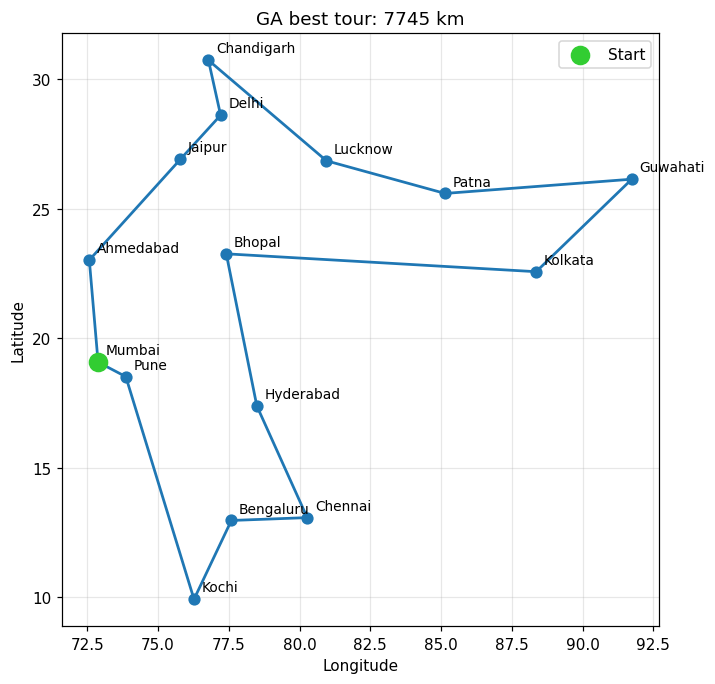
\includegraphics[width=0.48\textwidth]{figures/ga_route.png}\hfill
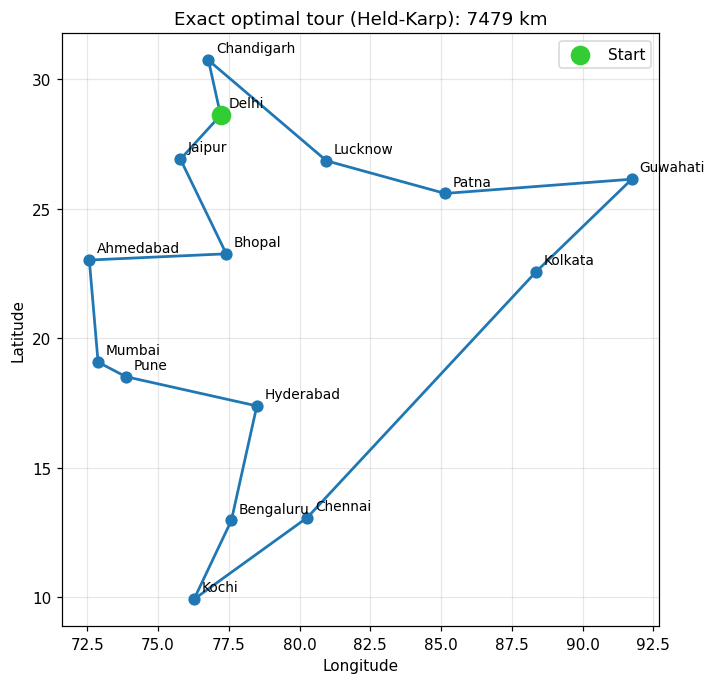
\includegraphics[width=0.48\textwidth]{figures/optimal_route.png}
\caption{Left: best tour of a single GA run (seed 42, 7745~km). Right: exact optimal tour from Held--Karp (7479~km).}
\label{fig:routes}
\end{figure}

Figure~\ref{fig:conv} shows convergence. The population average drops quickly in the first generations as
selection removes poor tours, while the best-so-far curve flattens once the population has converged.

\begin{figure}[H]
\centering
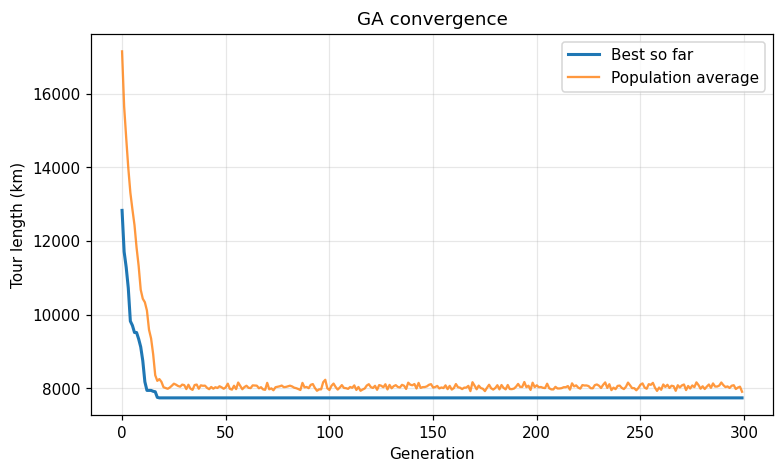
\includegraphics[width=0.8\textwidth]{figures/ga_convergence.png}
\caption{Convergence of the GA: best tour length so far and population average per generation.}
\label{fig:conv}
\end{figure}

\subsection{Comparison with baselines}
\begin{table}[H]
\centering
\caption{GA versus baselines. Random search uses the same budget of $150\times300=45{,}000$ evaluations.}
\label{tab:base}
\begin{tabular}{@{}lrr@{}}
\toprule
Method & Length (km) & Gap to optimum \\
\midrule
Random search (mean of 3)          & 9930.4 & 32.8\% \\
Nearest neighbour                  & 9169.4 & 22.6\% \\
Genetic Algorithm (mean of 10 runs) & 7526.9 & 0.6\% \\
Genetic Algorithm (best of 10 runs) & 7478.9 & 0.0\% \\
Exact optimum (Held--Karp)         & 7478.9 & 0.0\% \\
\bottomrule
\end{tabular}
\end{table}

The GA reached the exact optimum in 5 of 10 runs and was never far from it, while examining only 45{,}000 of
roughly $4.4\times10^{10}$ possible tours.

\subsection{Effect of mutation rate}
Each setting was run 8 times for 200 generations.

\begin{table}[H]
\centering
\caption{Final tour length by mutation rate (8 runs each).}
\label{tab:mut}
\begin{tabular}{@{}rrr@{}}
\toprule
Mutation rate & Mean length (km) & Best length (km) \\
\midrule
0.00 & 8079.0 & 7503.7 \\
0.05 & 7660.8 & 7478.9 \\
0.20 & 7532.2 & 7478.9 \\
0.50 & 7545.6 & 7478.9 \\
0.90 & 7478.9 & 7478.9 \\
\bottomrule
\end{tabular}
\end{table}

\begin{figure}[H]
\centering
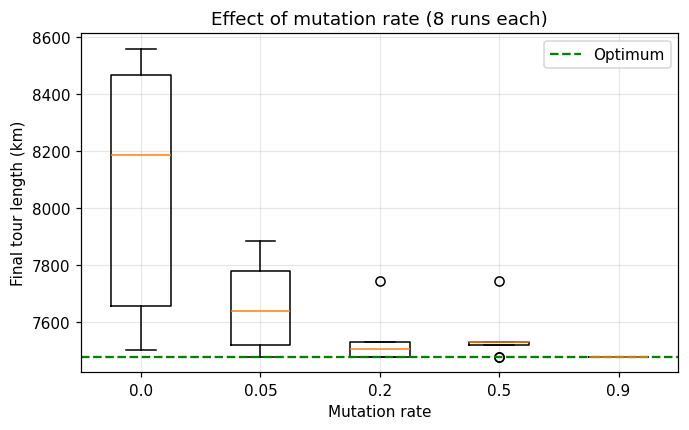
\includegraphics[width=0.7\textwidth]{figures/mutation_rate.png}
\caption{Spread of final tour lengths by mutation rate. The dashed line is the exact optimum.}
\label{fig:mut}
\end{figure}

With no mutation the GA performs worst: crossover only recombines genes already in the population, so diversity
collapses and the search stalls. In this experiment higher mutation rates did better, and the highest rate
tested (0.9) found the optimum in every run. Inversion is a gentle move, so it tolerates high rates; a more
disruptive operator would not.

\subsection{Effect of population size}
Every setting used the same budget of 45{,}000 evaluations, so smaller populations ran more generations.

\begin{table}[H]
\centering
\caption{Final tour length by population size at equal evaluation budget (8 runs each).}
\label{tab:pop}
\begin{tabular}{@{}rrrr@{}}
\toprule
Population & Generations & Mean length (km) & Best length (km) \\
\midrule
10  & 4500 & 7683.1 & 7532.3 \\
30  & 1500 & 7676.5 & 7478.9 \\
100 & 450  & 7598.8 & 7478.9 \\
300 & 150  & 7518.9 & 7478.9 \\
\bottomrule
\end{tabular}
\end{table}

\begin{figure}[H]
\centering
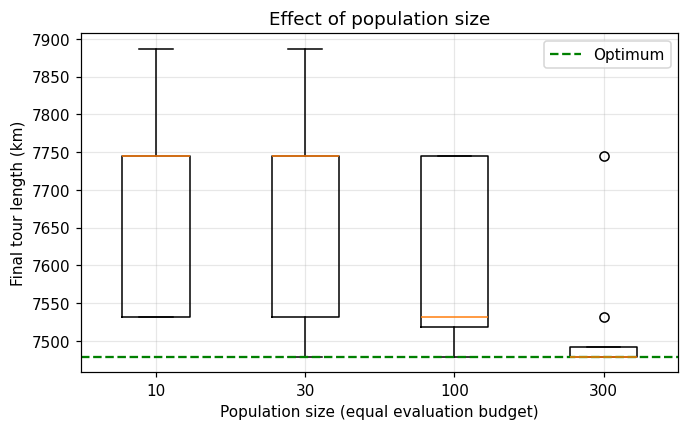
\includegraphics[width=0.7\textwidth]{figures/population_size.png}
\caption{Spread of final tour lengths by population size at equal evaluation budget.}
\label{fig:pop}
\end{figure}

Larger populations did better. A population of 10 loses diversity quickly, so running 4500 generations does not
help once it has converged, whereas 300 individuals keep more distinct partial routes alive for recombination.

% ---------------------------------------------------------------- 4
\section{Complexity Analysis}
Let $P$ be the population size, $G$ the number of generations and $n$ the number of cities.
\begin{itemize}[nosep]
  \item \textbf{GA time:} each generation evaluates $P$ tours at $O(n)$ each, and crossover and mutation are $O(n)$
        per child, giving $O(G\cdot P\cdot n)$.
  \item \textbf{GA space:} $O(P\cdot n)$ for the population.
  \item \textbf{Held--Karp:} $O(n^2 2^n)$ time and $O(n\,2^n)$ space.
\end{itemize}
The GA scales polynomially in $n$, whereas the exact method grows exponentially and is impractical beyond
roughly 25 cities.

% ---------------------------------------------------------------- 5
\section{Limitations}
\begin{itemize}[nosep]
  \item The GA gives no optimality guarantee; a single run can stall in a local optimum, as the seed-42 run did.
  \item Results depend on the parameters and the random seed, so they should be reported over repeated runs.
  \item Premature convergence occurs when population diversity is lost, especially with small populations or
        no mutation.
  \item The experiments use one 15-city instance with 8--10 runs per setting, so the parameter trends are
        indicative rather than conclusive.
\end{itemize}

% ---------------------------------------------------------------- 6
\section{Conclusion}
The GA found tours within 0.6\% of the exact optimum on average for a 15-city TSP and reached the optimum in
half of the runs, clearly outperforming random search and nearest neighbour at the same budget. The experiments
show that mutation is necessary to avoid stagnation and that larger populations make better use of a fixed
evaluation budget. Validating against Held--Karp turned a vague claim of a ``good solution'' into a measured
optimality gap.

\end{document}
